\section{Tests}
Several tests have been included in our assignment to test the functionality of our implemented functions. Also, new ones have been created to further test the functionality of our fasto-compiler.\\
For example, we have written the following test for the functionality of the \textit{or}-operator, which looks as so:\\
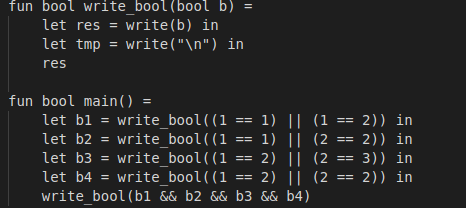
\includegraphics[width=\linewidth]{Materials/Tests/OrTest}
This test (alongside most others) suceed by matching expected input. In the case of the test above, the expected output, which it matches, looks like the following:\\
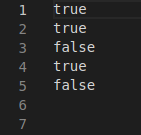
\includegraphics[width=0.4\linewidth]{Materials/Tests/OrExpected}\\
Some tests don't suceed however. This is on purpose, as many tests have been made (Those, which names end in "TypeChecker.fo") to test the implemented typechecker. These tests purposefully use nonsensical types (like using the \textit{or}-operator between integers or multiplying an int with a bool). The typechecker-test with regards to the \textit{or}-operator looks like so:\\
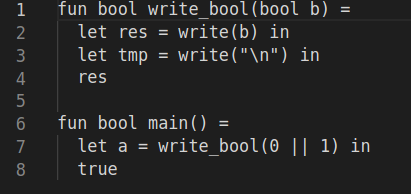
\includegraphics[width=\linewidth]{Materials/Tests/OrTypeCheck}\\
which fails since the \textit{or}-opetator expects two expressions of type Bool but are only given integers. Also, this test doubles as a reassurence that $0$ and $1$ aren't evaluated as \textit{false} and \textit{true}, respectively. 
